\chapter{Delta Smile Facial Survey Analyzerシステム}
%20191222 推敲1回目済み
\label{chap:aboutDSFSA}

本章では, 本研究の目的である笑顔からお互いを分析し, 人と人との繋がり作成を助長するシステムを作成のため,
データ収集およびデータ分析のためのツールDelta Smile Facial Survey Analyzer(以下DSFSA)について述べる.
はじめにシステムの大まかな流れを述べた後, 本システムの特徴および使用方法について述べる.


\section{DSFSAシステムの概要}
本システムは表情分析をするためのデータを収集・分析するためのツールである.
ユーザーの顔を検出し,トラッキングをしつつ,
ユーザーが中立の表情から笑顔になったタイミングを検出する.
各フレームごとに画像処理をして表情の分析を行い, 動画としてデータベースへ保存する.
Open FaceのFacial Action Units を使用して特徴量を算出した後,
データベースの中にある決まったフォーマットの笑顔の作り方動画を5種類選択し,ユーザーに表示する.
その際には, 顔の特徴点のみを描画した動画を表示することで表情の動き以外のバイアスを軽減する.
システムによって選択された動画を2つずつ表示し, ユーザーに比較をして,選んでもらうことで動画データに順位づけを行う.
ユーザーの表情データ, 選ばれたデータベース内の動画を分析した表情データ, および順位づけデータを使用して,
ユーザーの表情と, ユーザーの表情の観点から人を選ぶ嗜好との関連性を分析する.

\begin{figure}[htbp]
    \begin{center}
       \fbox{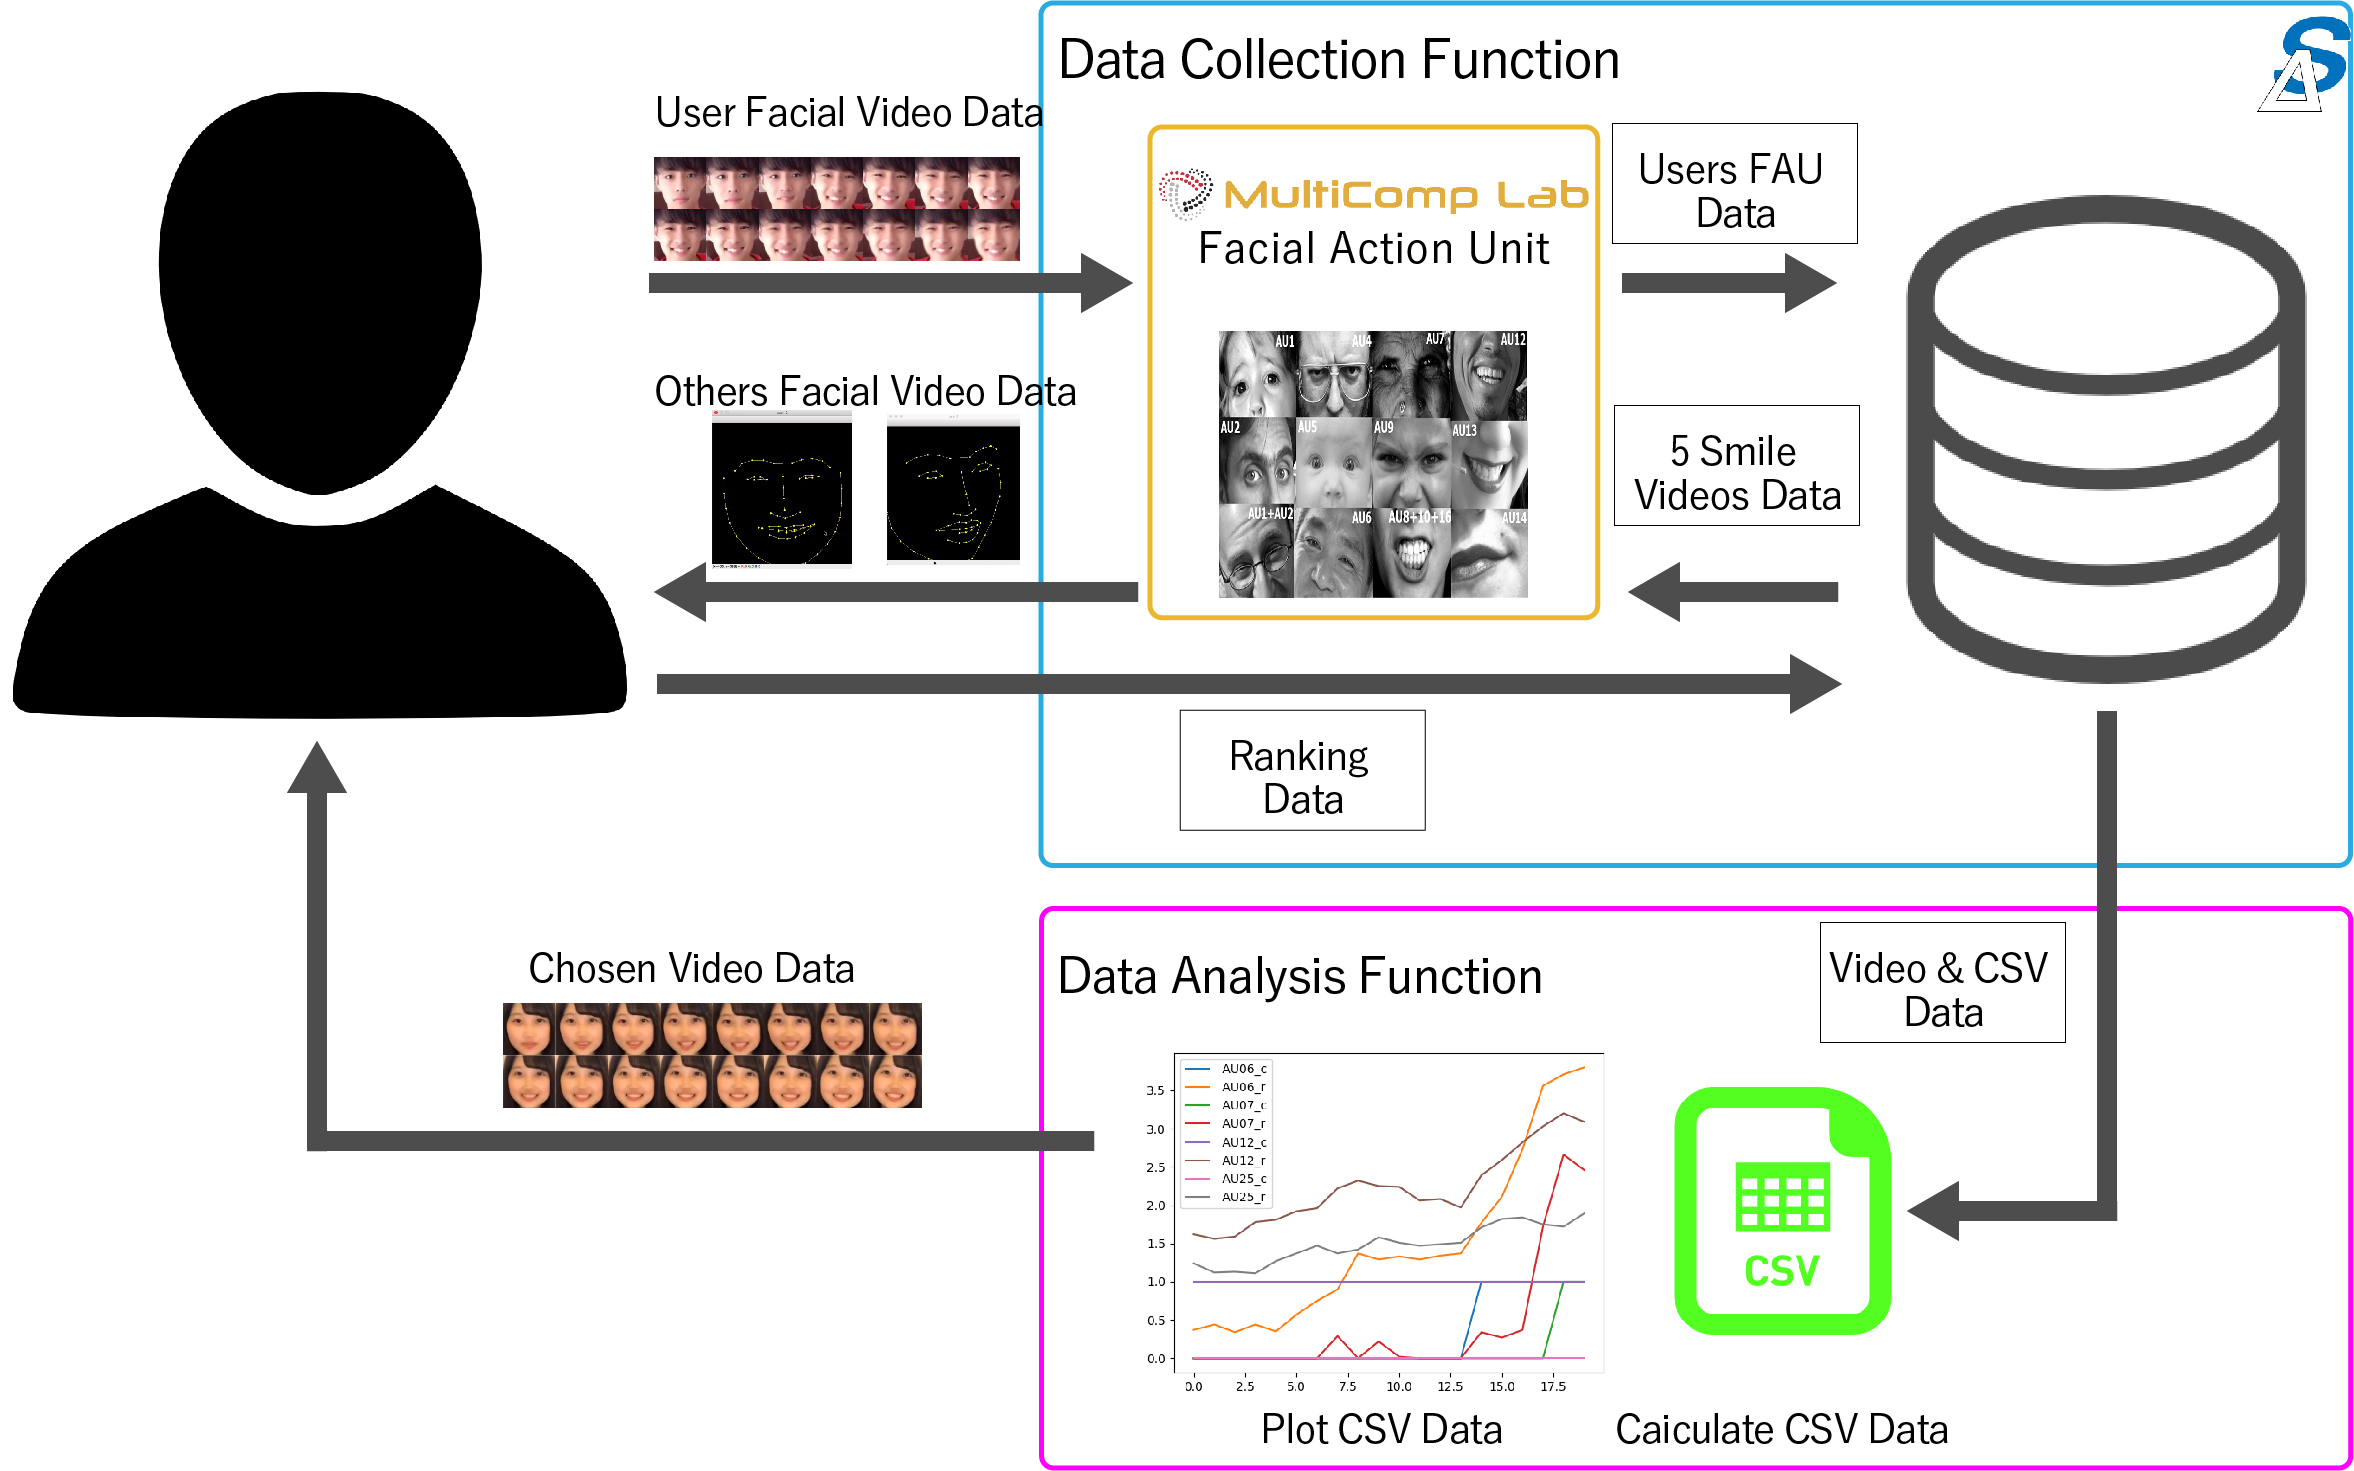
\includegraphics[width=150mm,bb=0 0 2354 1471]{system_flow.jpg}}
    \end{center}
    \caption{システムフロー}
    \label{fig:system_architecture}
\end{figure}


\section{DSFSAの特徴}
本システムの特徴は, 中立と笑顔の表情を部分的に切り取った断片的な画像データではなく,
動画の形を採用することで表情の遷移を時系列データで, 笑顔の作り方を記録し,分析することが可能な点である.
SONYが開発したスマイルシャッターのように笑顔になったタイミングをキャプチャーするシステムなど,
笑顔のタイミングのみにフォーカスをあてた研究やサービス,笑顔のタイミングのみを切り取って表情分析をする研究は盛んに行われているが,
動画など時系列データを使用した表情分析系の研究はまだ少ない.
Bruce \& Youngらは表情表出の時間的特性が感情の認知に影響を及ぼす結果を得ており\cite{kokada},
感情の認識においては動画像解析による動的な特徴を抽出することが望ましいと述べている\cite{yukitakahashi}.
本システムにおいては, 中立表情から笑顔になるまでの表情の遷移を記録し,
顔のパーツの動き, 筋肉の動きを数値化することが可能である.
数値化可能な値は, 顔のパーツの位置, 動きがあるかないかの2極値, そして動きの強度である.

\section{DSFSAの使用方法}
2つのモードを使いわけて, 笑顔の作り方を記録した動画データを作成することおよび顔パーツの動きを
数値化することが可能である.
また, 中立の表情から笑顔になるタイミングを記録した動画データのことを以下では笑顔動画データとする.
\subsection{動画から笑顔動画データ作成および数値化}
人が映った既存の動画データから, 笑顔動画データを作成することが可能である.
ユーザーに表示するための笑顔動画データを作成, 収集するために使用するモードである.
特にユーザーに対してシステムを使用する前に, データベースにデータが空の状態では順位づけをする
ことができないため, 主に初期状態から運用可能状態にする用途がこのモードにはある.
%ここ膨らます
\subsection{ユーザー表情の笑顔動画データ作成および数値化}
実際にユーザーの表情の動きをトラッキングして, 笑顔動画データを作成することが可能である.
表情と嗜好の関係性をするためのデータを収集およびユーザーの笑顔動画データをデータベースに
保存するためのモードである.
主なモードであり, ユーザーの情報を入力して, 分析および出力, 保存まで全ての一連の流れを
実行・処理することが可能である.
%ここ膨らます

\section{まとめ}
本章では, 笑顔動画データ作成および収集, 数値化を行う本システムの概要について述べた.
ついで, 本システムの特徴および使用方法について説明をした.
次章では, Delta Smile Facial Survey Analyzer システムの設計について述べる.
